%\title{Approximation for Piecewise Linear Functions}

%For many continuous probabilistic planning problems it is useful to describe transition or reward functions as piecewise linear functions of problem variables. This class of functions can be represented efficiently in linear eXtended Algebraic Decision Diagrams (LinXADDs). However, as the complexity of the function grows, the number of different cases and linear pieces may become intractably large even with few variables. A practical approach to tackle larger problems is to make approximations with a limited error, reducing the number of cases and of different linear functions. Our goal here is to describe an efficient method for obtaining the best linear approximation, and the error incurred, for two distinct linear functions defined on cases.

%\section{Problem and Solution} 
%\label{probSol} 
In this section, we present a novel method for approximating piecewise linear functions. The goal of this algorithm is to reduce the number of partitions of a piecewise linear function represented in case form. This represents the ability to automatically identify and remove locally unimportant constraints, whose removal results in a small change in the represented function in exchange for a significant improvement in the efficiency of computations with these functions. XADDs already permit compactness by exploring variable and context independencies, so our approach is to merge terminal nodes as a way of reducing the number of dependencies that need to be represented. Thus, the most important step in the approximation algorithm is the optimal merging of linearly constrained linear functions. 

Since boolean variables are either mutually independent or exclusive (the negated version of them), and don't affect directly the continuous domain of the functions in terminal nodes, our approximation works independent of the boolean variables, so we will consider piecewise linear functions whose partitions are defined only with linear inequalities. We observe that regions defined by conjunctions of linear inequalities are (possibly unbounded) polytopes and a disjunction of formulas is the union of the  regions defined by each sub formula, so that a generic formula $\phi$ of linear inequalities is equivalent to a region defined by a union of polytopes $\theta$. We denominate $Poly(\phi)$ the set of all polytopes generated expanding disjunctions of $\phi$.
Second, since we are only concerned for linear functions, $f$ must be of the form $f(\vec{x}) = \vec{c}\cdot \vec{x}_0$ , where $\vec{x}_0$ denotes the extended vector $(1,\vec{x})$ to include the constant term $c_0$ of $f$. This means that an arbitrary linear function on a set of variables is equivalent (isomorph) to a vector $\vec{c}$ of linear variables, called parameters of $f$.
Next we proceed to define the crucial step for the approximation algorithm, optimal merging of linear case functions.

\subsection{ Optimal merging of linear case functions}
More formally, given two case linear functions $L_1 = ( f_1, \phi_1 )$ and $L_2 = ( f_2, \phi_2 )$, our goal is to determine the best linear case approximation of $L_1$ and $L_2$. As it must represent  $L_1$ and $L_2$, the solution must be defined in both regions, therefore of the form $L^* = (f^*,\phi_1 \cup  \phi_2)$ . In this case, we must find a linear function $f^*$ that minimizes approximation error $E$, defined as the maximum  error of replacing both $f_1$ in $\phi_1$ and $f_2$ in $\phi_2$ by $f^*$:

\begin{equation} E(f) = \max ( |f - f_1|_{\phi_1} , |f - f_2|_{\phi_2} ) \label{maxstep} \end{equation}
\begin{equation} f^* = \argmin_f E(f)  \label{minstep} \end{equation}

Note that the absolute value in~\ref{maxstep} is equivalent to max of two linear functions, e.g. $|f - f_1| = max ( f - f_1, f_1 - f)$. Moreover, each of these partition $\phi_i$ constrained max is equivalent to the max in all polytopes $\theta_{1{i_1}}$ of $\phi_i$. With this, we can rewrite the error $E$ as the maximum of a finite number of errors restricted to polytopes, e.g.:
{%\footnotesize 
\begin{align}
\footnotesize
 e_{1{i_1}}(f) = max_{\vec{x} \in \theta_{1{i_1}}} (f - f_1)(\vec{x}) \forall \theta_{1{i_1}} \in Poly(\phi_1) \nonumber\\
 e_{2{i_2}}(f) = max_{\vec{x} \in \theta_{2{i_2}}} (f - f_2)(\vec{x}) \forall \theta_{2{i_2}} \in Poly(\phi_2) \nonumber\\
 e_{1{i_3}}(f) = max_{\vec{x} \in \theta_{1{i_3}}} (f_1 - f)(\vec{x}) \forall \theta_{1{i_3}} \in Poly(\phi_1) \nonumber\\
 e_{2{i_4}}(f) = max_{\vec{x} \in \theta_{2{i_4}}} (f_2 - f)(\vec{x}) \forall \theta_{2{i_4}} \in Poly(\phi_2)\nonumber\\
E(f) = max_{k=1..K} (e_k(f)) \nonumber
\end{align}
where $K$ is the total number of polytopes and e$ _k$ is an enumeration of all $e_{nj}, n = 1,2; j $ is index of a polytope.
}

This bilinear piecewise optimization problem is very complex, including minimization on the parameters $\vec{c}$, maximization on the variables $\vec{x}$ and case max between the polytope maximums, thus we can break it down to a three step optimization problem: 

(i) There are linear constrained bilinear functions $L_{k}(f,\vec{x},\phi_k) =  ( l_k(\vec{c},\vec{x}) ,\phi_k)$ depending on both the domain variables $\vec{x}$ and parameter variables $\vec{c}$, defined in $\phi_k$ such as $ ( (f - f_1)(\vec{x}),\phi_1) = ( (\vec{c}-\vec{c_1})\cdot\vec{x}, \phi_1)$. The innermost optimization step is the constrained maximization of this bilinear function on the domain variables.
\begin{equation} e_k(f) = max_{\vec{x}} ( L_k(f,\vec{x},\phi_k) ) = max_{ {\vec{x}} \in \phi_k} (l_k (\vec{c}, \vec{x}) ) \label{step1} \nonumber \end{equation}

(ii)There is a case max in a finite group of this linear constrained bilinear functions :
\begin{equation} E(f) = \max_{k=1..K} ( max_{\vec{x}} ( L_k(f,\vec{x},\phi_k) )) = \max_{k=1..K} ( e_k(f)) \label{step2}  \nonumber \end{equation}

(iii)Finally, this case max is minimized in terms of the parameters $\vec{c}$ as in ~\ref{minstep}:
\begin{equation} e_k = max_{\vec{x} } \end{equation}

In order to solve it we propose an elaborate iterative constraint generation based algorithm. The details of the algorithm will be exposed in the next section, but first we present a quick outline: 

First, the algorithm will iterate between two phases, one for the maximization and one for the minimization. Second, on each phase a relaxed problem will be solved using the result from the previous phase. Third, when a phase gives the same return twice, the algorithm has converged.

In the maximization phase, we will always assume a fixed $f$, and thus the maximization of the bilinear functions $L_{k}(f,\vec{x},phi_k$ for each linear case function will be a linear constrained linear program, solved efficiently by a LP solver. The optimal values are upper bounds on the actual minimal error in each polytope. More importantly, the vertexes that reach this optimal values are the points of the polytope that maximize the bilinear function for this function $f$ and thus are important points to which the minimization must attempt to reduce the error (in fact reducing the error in any set of points that doesn't contain this point won't change the maximal error, and thus won't improve our solution.

In the minimization phase, we will solve a relaxation of~\ref{minstep}, where in each linear constrained bilinear function $e_k$ the maximal error in the polytope $\theta_k$ is replaced by the greater of the error in a finite set of points. More specifically, we only minimize the greatest of the error on points found in the maximization phase. This changes the piecewise bilinear problem into a linear program with the objective to be minimized is the error, and linear constraints encode that this error must be greater than the error on any of the previously obtained points. Solving this minimization yields a new solution $f$ whose error is a lower bound on the actual minimal error in each of these points (this $f$ may have to be modified to minimize the error in more points in the next iterations, but this can only lead to increasing the error in the points that were present in this iteration. Put simply, adding more constraints cannot improve the optimal value of solution for a linear program.

Finally, we can see why if either of the phases do not produce changes the solution must be optimal for the piecewise bilinear problem as a whole. In the case of the maximization, if all the points generated (in all polytopes) were already in the previous minimization phase than the error in any of these cannot be reduced, and since this points include the points of maximal error in all polytopes the actual global maximal error is achieved in one of them, and therefore no solution can have a better maximal error than the current $f$. Similarly, if a repeated value function $f$ is produced in the minimization this means that this function already minimized the error in its greatest error points (added in the previous maximization) therefore no other function can reduce the error in one of this points and these include the maximal error, se the maximal error cannot be reduced, thus we have an optimal solution.

\section{Algorithm}
We will define an iterative algorithm using linear solvers in two different steps. Algorithm \ref{alg:glo} is the main method that solves the approximation problem using the functions $MAX\_ERROR$ and $BEST\_APPROX$, which use a linear programming, $LP\_Solve($ max or min$, objective, constraints)$.

\begin{algorithm}[!h]
\dontprintsemicolon
\KwIn{A pair of case linear functions $L_1 = ( f_1, \phi_1 )$ and $L_2 = ( f_2, \phi_2 ).$}
\KwOut{$L^* = (f^*,\phi_1 \cup  \phi_2)$ that best approximates $L_1$ and $L_2$.}
$f \gets 0$\;
$points \gets \emptyset$\;
$new\_points = MAX\_ERROR(f, L_1,L_2)$\;
\While{$new\_points \not \subset points$} {
	$points = points \cup new\_points$\;
	$f = BEST\_APPROX(f_1,f_2,points)$\;
	$new\_points = MAX\_ERROR(f, L_1,L_2)$\;}
\Return{$f$}\;
\caption{{\sc Constraint Generation MiniMax} finds the best case linear function}
\label{alg:glo}
\end{algorithm}

\subsection{MAX\_ERROR}
We show that for a given $f$ the internal maximization can be done with four linear optimizations:

Remembering $ |f - f_1| = max (f-f_1,f_1-f)$ we get that our error is the greater of four similar restricted maximizations.
$$ E(f) =\max \left( max_{x\in \phi_1} (f - f_1) (x),
max_{x\in \phi_1} (f _1- f) (x),
max_{x\in \phi_2} (f - f_2) (x),
max_{x\in \phi_2} (f_2 - f) (x)
\right)$$
For simplicity we will inspect one of these, considering that our functions are all linear, we can use:
$$ f = \sum_{i=0}^n w_i x_i,  \mbox{\rule{1cm}{0cm}} 
f_1 = \sum_{i=0}^n \alpha_i^1 x_i$$

$$max_{x\in \phi_1} (f _1- f) (x) = max_{x\in \phi_1}\sum_{i=0}^n (w_i- \alpha_i^1) (x) $$
which is a linear optimization problem for x, resulting in the maximum error and the solution $x^*$  where this error is maximum.
This is illustrated in algorithm \ref{alg:max}.

\begin{algorithm}[!h]
\dontprintsemicolon
\KwIn{Two case linear functions $L_1 = ( f_1, \phi_1 ), L_2 = ( f_2, \phi_2 )$ and an approximation $f$ }
\KwOut{Four points where each of the four errors is maximal.}
$p_1 \gets LP\_Solve(max _x, f-f_1,\phi_1)$\;
$p_2 \gets LP\_Solve(max_x, f_1-f,\phi_1)$\;
$p_3 \gets LP\_Solve(max_x, f-f_2,\phi_2)$\;
$p_4 \gets LP\_Solve(max_x, f_2-f,\phi_2)$\;
\Return{$\{p_1,p_2,p_3,p_4\}$}\;
\caption{{\sc MAX\_ERROR} finds the points of maximum error}
\label{alg:max}
\end{algorithm}

\subsection{BEST\_APPROX}
We show that this maximum error points induce constraints for a linear relaxation of the minimization problem.
A relaxation of the minimization problem is instead of minimizing the maximum error in all points of $\phi_1 \cup \phi_2$, minimizing the error on two finite set of points $X^1 = \{ x^1_1, ..., x^1_{m_1} \} \subset   \phi_1$ and $X^2 = \{ x^2_1, ..., x^2_{m_2} \} \subset   \phi_2$
	
$$ \tilde{E}(f) =\max \left( (f - f_1) (x^1_1), ... , (f - f_1) (x^1_{m_1}),  (f _1- f) (x^1_1), ... ,  (f - f_2) (x^2_1), ... , (f_2 - f) (x^2_{m_2})
\right)$$


$$\tilde{f} = argmin_w \tilde{E}(f) $$
or, converting the max into constraints by adding an artificial variable $Z$.

$$\tilde{f} = argmin_{f,Z}  Z $$
s.t. 
$$
	\begin{array}{llll}
		Z & \geq & (f - f_1) (x^1_j) & \mbox{for } j = 1,...m_1\\
		Z & \geq & (f_1 - f) (x^1_j) & \mbox{for } j = 1,...m_1\\
		Z & \geq & (f - f_2) (x^2_k) & \mbox{for } k = 1,...m_2\\
		Z & \geq & (f_2 - f) (x^2_k) & \mbox{for } k = 1,...m_2\\
	\end{array}
$$

This is now a linear problem in the coefficients of $f$, the solution Z is the error incurred in the approximation. This is illustrated in algorithm \ref{alg:best}.

\begin{algorithm}[!h]
\dontprintsemicolon
\KwIn{Two case linear functions $L_1 = ( f_1, \phi_1 ), L_2 = ( f_2, \phi_2 )$ and a set of $points$ where to find the best approximation for them}
\KwOut{Best linear approximation for both $f$.}
$constr \gets \emptyset$\;
\For {$p \in points$}{ 
	\If {$p \in \phi_1$}{
		$constr \gets constr \cup \{ (Z \geq (f - f_1) (p)), (Z \geq (f_1 - f) (p) )\} $}\;
	\If {$p \in \phi_2$}{
		$constr \gets constr \cup \{ (Z \geq (f - f_2) (p)), (Z \geq (f_2 - f) (p) )\} $}\;
}\;
$f \gets LP\_Solve(min_{f,Z}, Z, constr)$\;	
\Return{$f$}\;
\caption{{\sc BEST\_APPROX} finds the best approximation on points}
\label{alg:best}
\end{algorithm}

\section{Conclusion}
We have presented an iterative constraint generation method for obtaining the best case linear function for approximating two other case linear functions. The algorithm has implemented on the java XADD package, was used in small tests for pruning specific trees and will soon be tested on diagrams from solution of continuous MDPs. 
\newpage
\appendix
\section{Definitions} 
\label{appA} 

First we give the basic definitions of our mathematical model.\\
Let  $\mathbb{X}$ be a set of real valued variables: $\mathbb{X} = \{ x_1, x_2, ... , x_n\ | x_i \in \mathbb{R}, \forall i\}$\\
A linear function $f: \mathbb{R}^n \rightarrow \mathbb{R}$ over $\mathbb{X}$ is a linear combination of the variables and a constant 
$$f(x) = \sum_{i=0}^n { \alpha_i x_i}$$ where $\alpha_i \in \mathbb{R}$ and $x_0$ equals $1$.\\
A linear constraint is a region of $\mathbb{R}^n$ defined by the signal of a linear function $f$:
$$c = \{	x \in \mathbb{R}^n | f(x) \geq 0 \} $$
A linear case $\phi$ is the region defined by $m \in \mathbb{N}^+$ linear constraints $c_1, c_2, ... c_m$:
$$ \phi =c_1 \cap c_2 \cap ... \cap c_m $$

A case linear function is a pair $(f, \phi)$, where $f$ is a linear function and $\phi$ is a linear case.  $(f, \phi)$ denotes the partial function equal to $f$ in $\phi$ and undefined elsewhere.

A piecewise linear function is a function $f: \mathbb{R}^n \rightarrow \mathbb{R}$ defined by joining different case linear functions with exclusive cases:
$$ f = 
\left\{
	\begin{array}{ll}
		\phi_1 : & f_1(x)\\
		\phi_2 : & f_2(x)\\
		... & \\
		\phi_m : & f_m(x)\\
	\end{array}
\right.
$$
where $\phi_i \cap \phi_j = \emptyset$ if $i \neq j$

\section{Underconstrained Problem} 
\label{appB} 

A clear example of a function where approximation can be helpful is a regular difference step function, as the one in picture \ref{stepf}. 
\begin{figure}[!h]
\center
\fbox{Missing}%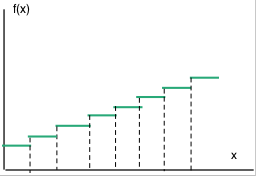
\includegraphics[scale=0.9]{Figures/step.png}
\caption{A linearizable step function.}
\label{stepf} 
\end{figure}

For this function it seems clear that with a small error, a much simpler representation can be achieved by modifying the linear function and merging the regions. We would like to represent it concisely as in figure \ref{steplin}.
\begin{figure}[h]
\center
\fbox{Missing}%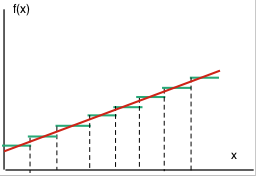
\includegraphics[scale=0.9]{Figures/steplin.png}
\caption{An approximation reducing the number of cases.}
\label{steplin} 
\end{figure}
Considering the complexity of comparing multiple functions our approach would be to compare and merge the regions pairwise, making successive merges until all regions have collapsed, in a procedure as shown in picture \ref{steplining}. While our merging algorithm minimizes the error in each merge the total error is evaluated as the sum of errors incurred in successive merges, and is not explicitly minimized.

\begin{figure}[!h]
\centering
\begin{minipage}{.7\textwidth}
  \centering
  \subfigure[Original] {
	\fbox{Missing}%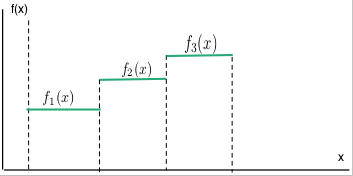
\includegraphics[scale=0.75]{Figures/step1.png}
	\label{step1}
  }
\end{minipage}
\begin{minipage}{.7\textwidth}
\centering
\subfigure[Step1] {
	 \fbox{Missing}%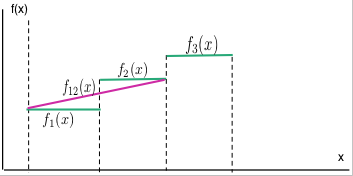
\includegraphics[scale=0.75]{Figures/step12.png}
	\label{step2} 
}
\end{minipage}
\begin{minipage}{.7\textwidth}
\centering
\subfigure[Step2]{
	 \fbox{Missing}%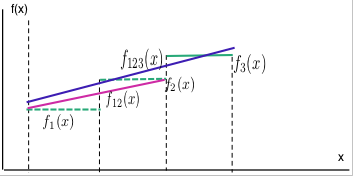
\includegraphics[scale=0.75]{Figures/step123.png}
	 \label{step2}
}
\end{minipage}
\caption{ Making the approximation by successive merging}
 \label{steplining}
\end{figure}

Therefore, while making experiments it became clear that when merging linear functions with the same angular coefficient, as the step function case, the problem of minimizing the maximal error has various solutions, out of which our algorithm will arbitrarily choose one. An example is depicted in figure \ref{steplin2}. Both functions $f_1(x)$ and $f_2(x)$ approximate the step function optimally according to the maximum error so either may be chosen by our algorithm.This reveals that the problem specified earlier, of finding the best linear case approximation for two linear case functions is possibly underspecified.  Its is suggested that since $f_2(x)$ yields a smaller average error than $f_1(x)$ it could be used to improve the approximation. Minimizing other forms of errors would avoid this underspecification. Another concern is if choosing the appropriate optimal function will lead to a better total error, as the propagations of errors for successive merges may not provide the overall best approximation.
\begin{figure}[h]
\center
\fbox{Missing}%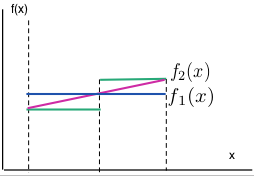
\includegraphics[scale=0.9]{Figures/step2lin.png}
\caption{Two optimal MaxError approximations.}
\label{steplin2} 
\end{figure}
